% This example is meant to be compiled with lualatex or xelatex
% The theme itself also supports pdflatex
\PassOptionsToPackage{unicode}{hyperref}
\documentclass[aspectratio=1610, 12pt]{beamer}

% Warning, if another latex run is needed
% \usepackage[aux]{rerunfilecheck}

% just list chapters and sections in the toc, not subsections or smaller
\setcounter{tocdepth}{1}

%------------------------------------------------------------------------------
%------------------------------ Fonts, Unicode, Language ----------------------
%------------------------------------------------------------------------------
\usepackage{fontspec}
\defaultfontfeatures{Ligatures=TeX}  % -- becomes en-dash etc.

% german language
\usepackage{polyglossia}
\setdefaultlanguage{german}

% for english abstract and english titles in the toc
\setotherlanguages{english}

% intelligent quotation marks, language and nesting sensitive
\usepackage[autostyle]{csquotes}

% microtypographical features, makes the text look nicer on the small scale
\usepackage{microtype}

%------------------------------------------------------------------------------
%------------------------ Math Packages and settings --------------------------
%------------------------------------------------------------------------------

\usepackage{amsmath}
\usepackage{amssymb}
\usepackage{mathtools}
\usepackage{bbold}

% Enable Unicode-Math and follow the ISO-Standards for typesetting math
\usepackage[
  math-style=ISO,
  bold-style=ISO,
  sans-style=italic,
  nabla=upright,
  partial=upright,
]{unicode-math}
\setmathfont{Latin Modern Math}

% nice, small fracs for the text with \sfrac{}{}
\usepackage{xfrac}


%------------------------------------------------------------------------------
%---------------------------- Numbers and Units -------------------------------
%------------------------------------------------------------------------------

\usepackage[
  locale=DE,
  separate-uncertainty=true,
  per-mode=symbol-or-fraction,
]{siunitx}
\sisetup{math-micro=\text{µ},text-micro=µ}
% \sisetup{tophrase={{ to }}}
%------------------------------------------------------------------------------
%-------------------------------- tables  -------------------------------------
%------------------------------------------------------------------------------

\usepackage{booktabs}       % \toprule, \midrule, \bottomrule, etc

%------------------------------------------------------------------------------
%-------------------------------- graphics -------------------------------------
%------------------------------------------------------------------------------

\usepackage{graphicx}
%\usepackage{rotating}
\usepackage{grffile}
\usepackage{tikz}
\usepackage{circuitikz}
\usepackage{tikz-feynman}
\usepackage{subcaption}

% allow figures to be placed in the running text by default:
\usepackage{scrhack}
\usepackage{float}
\floatplacement{figure}{htbp}
\floatplacement{table}{htbp}

% keep figures and tables in the section
\usepackage[section, below]{placeins}

% smileys
\usepackage{MnSymbol,wasysym}

%------------------------------------------------------------------------------
%---------------------- customize list environments ---------------------------
%------------------------------------------------------------------------------

\usepackage{enumitem}
\usepackage{listings}
\usepackage{hepunits}

\usepackage{pdfpages}
%------------------------------------------------------------------------------
%------------------------------ Bibliographie ---------------------------------
%------------------------------------------------------------------------------

\usepackage[
  backend=biber,   % use modern biber backend
  autolang=hyphen, % load hyphenation rules for if language of bibentry is not
                   % german, has to be loaded with \setotherlanguages
                   % in the references.bib use langid={en} for english sources
]{biblatex}
\addbibresource{references.bib}  % the bib file to use
\DefineBibliographyStrings{german}{andothers = {{et\,al\adddot}}}  % replace u.a. with et al.


% Load packages you need here
% \usepackage{polyglossia}
% \setmainlanguage{german}

\usepackage{csquotes}


% \usepackage{amsmath}
% \usepackage{amssymb}
% \usepackage{mathtools}

\usepackage{hyperref}
\usepackage{bookmark}

% load the theme after all packages

\usetheme[
  showtotalframes, % show total number of frames in the footline
]{tudo}

% Put settings here, like
\unimathsetup{
  math-style=ISO,
  bold-style=ISO,
  nabla=upright,
  partial=upright,
  mathrm=sym,
}

% \setbeamertemplate{itemize item}{\scriptsize$\blacktriangleright$}
% \setbeamertemplate{itemize subitem}{\scriptsize$\blacktriangleright$}

%Titel:
\title{Gamma-Spectroscopy}
%Autor
\author[N.Breer]{Nils Breer}
%Lehrstuhl/Fakultät
\institute{Fakultät Physik}
%Titelgrafik muss ich einfueren!!!
%\titlegraphic{\includegraphics[width=0.3\textwidth]{content/Bilder/interferenz.jpg}}
\date{12.07.2022}

\begin{document}
\maketitle

\begin{frame}\frametitle{Agenda}
  \begin{itemize}
    \item What is gamma spectroscopy?
    \item Interactions in the Spectrum
    \item Detectorsystems
    \item Applications
  \end{itemize}
\end{frame}

\begin{frame}\frametitle{What is gamma spectroscopy?}
  \begin{itemize}
    \item \textbf{studies of energy spectra of gamma rays}
    \item spectrum used to determine quantity and identity of $\gamma$-emitters
    \item gamma ray sources emitters on earth, astrophysical sources
  \end{itemize}
\end{frame}

\begin{frame}\frametitle{Interaction of $\gamma$-rays with matter}
  \begin{columns}
    \begin{column}[c]{0.48\textwidth}
      \begin{figure}
        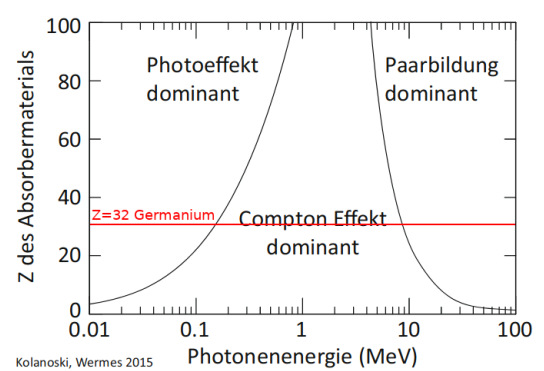
\includegraphics[width=\textwidth]{plots/z_depend.png}
        \caption{atomic number Z against photon energy E.}
      \end{figure}
    \end{column}
    \begin{column}[c]{0.48\textwidth}
      \begin{itemize}
        \item processes above ionization threshold
        \item Gamma ray absorption \to intensity loss
        \item Material thickness dependend intensity: $N(D) = N_0 e^{-\mu D}$
        \item D: thickness, $\mu$: absoption coefficient, $N_0$: initial intensity
      \end{itemize}
    \end{column}
  \end{columns}
\end{frame}

\begin{frame}\frametitle{Photoeffect}
  \begin{columns}
    \begin{column}[c]{0.48\textwidth}
      \begin{figure}
        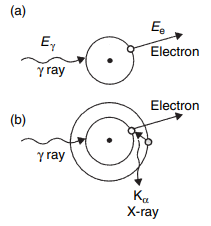
\includegraphics[width=0.9\textwidth]{plots/photo_abs.png}
        \caption{photo peak}
      \end{figure}
    \end{column}
    \begin{column}[c]{0.48\textwidth}
      \begin{itemize}
        \item $E_\gamma < $ several 100 keV
        \item ionizing bound electron (K-shell)
        \item $\gamma + atom \to atom^{+} + e^{-}$
        \item hole is filled with electrons from higher shells recursively
        \item energy diff. release as x-rays characteristic
        \item rarely: photon leaves absorber. often excite more electrons inside
        \item K-L-M-absorption edge: Quantumenergy enough to release bound electron from given shell
      \end{itemize}
    \end{column}
  \end{columns}
\end{frame}

\begin{frame}\frametitle{Compton scattering}
  \begin{columns}
    \begin{column}[c]{0.48\textwidth}
      \begin{figure}
        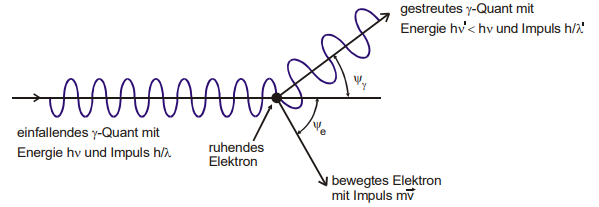
\includegraphics[width=\textwidth]{plots/compton.png}
        \caption{compton continuum}
      \end{figure}
    \end{column}
    \begin{column}[c]{0.48\textwidth}
      \begin{itemize}
        \item main interaction (100 keV < E < 5 MeV)
        \item inelastic scattering
        \item photons only transfers an energy fraction
        \item cannot view full spectrum \frownie{}
      \end{itemize}
    \end{column}
  \end{columns}
\end{frame}

\begin{frame}\frametitle{Compton scattering}
  \begin{columns}
    \begin{column}[c]{0.48\textwidth}
      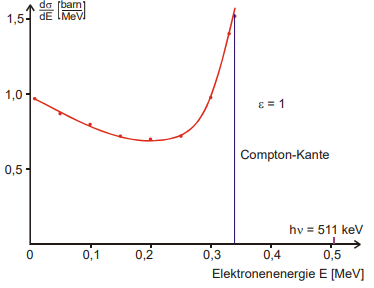
\includegraphics[width=\textwidth]{plots/compton_kante.png}
    \end{column}
    \begin{column}[c]{0.48\textwidth}
      \begin{itemize}
        \item non-isotropic angular distribution
        \item $E_\gamma\prime = \frac{E_\gamma}{1 + \left( \frac{E_\gamma}{511 keV} (1 - cos\theta)\right)}$
        \item $E_{e^-} = E_\gamma \left( \frac{\frac{E_\gamma}{511 keV}(1 - cos\theta)}{1 + \frac{E_\gamma}{511 keV}(1 - cos\theta)} \right)$
        \item extreme cases: backward scattering, light graze
      \end{itemize}
    \end{column}
  \end{columns}
\end{frame}

\begin{frame}\frametitle{Pair production}
  \begin{columns}
    \begin{column}[c]{0.48\textwidth}
      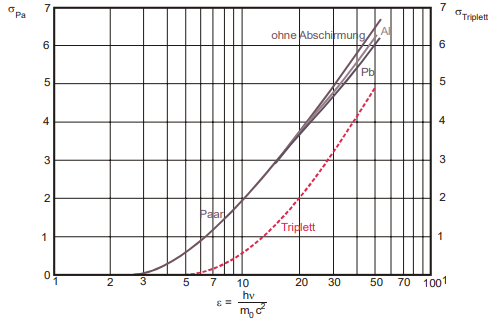
\includegraphics[width=\textwidth]{plots/pair_triplett.png}
    \end{column}
    \begin{column}[c]{0.48\textwidth}
      \begin{itemize}
        \item photon produces e+e- pair if E is high enough (5 MeV < E < 10 MeV)
        \item occurs in proximity of nucleus/scattering partner
        % \item in restframe photon mass = 0, lepton mass > 0; someone needs to take the momentum
        \item photon line visible if both leptons are absorbed;
        \item annihilation peak : 511 keV (e- mass) or doubled for both
        \item single- and double-escape peaks
      \end{itemize}
    \end{column}
  \end{columns}
\end{frame}

\begin{frame}\frametitle{Band structure}
  \begin{columns}
    \begin{column}[c]{0.48\textwidth}
      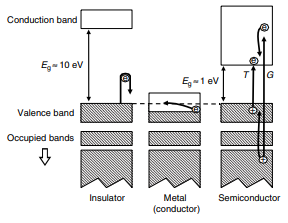
\includegraphics[width=\textwidth]{plots/bands.png}
    \end{column}
    \begin{column}[c]{0.48\textwidth}
      \begin{itemize}
        \item electrons in discrete/precise energy bands
        \item valence band: outer band for chemical reactions; most inhibited
        \item conduction band: migration of electrons
      \end{itemize}
    \end{column}
  \end{columns}
\end{frame}

\begin{frame}\frametitle{Mobility of "Holes"}
  \begin{columns}
    \begin{column}[c]{0.48\textwidth}
      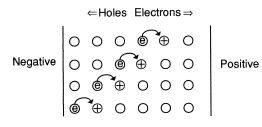
\includegraphics[width=\textwidth]{plots/holes.png}
    \end{column}
    \begin{column}[c]{0.48\textwidth}
      \begin{itemize}
        \item positive charge $\equiv$ hole in the band
        \item measuring the energy relies on separating the charge carriers
        \item electrons from valence band filling holes -> effective moving
        \item -> conductivity
      \end{itemize}
    \end{column}
  \end{columns}
\end{frame}

\begin{frame}\frametitle{Creation of charge carriers}
  \begin{columns}
    \begin{column}[c]{0.48\textwidth}
      \begin{itemize}
        \item excite electrons from low bands through high energies (E > $E_\text{therm}$)
        \item redistribution of electrons-holes throughout energy-bands
        \item holes: top of valence band
        \item electrons: bottom of conduction band
        \item external field: charge carriers migrate towards respective electrode
      \end{itemize}
    \end{column}
    \begin{column}[c]{0.48\textwidth}
      \begin{itemize}
        \item number of electron-hole pairs $n = E_\text{abs} / \epsilon$
        \item $\epsilon$: average energy needed to create electron hole pair
        \item $E_\text{abs}$: absorbed gamma ray energy
      \end{itemize}
    \end{column}
  \end{columns}
\end{frame}

\begin{frame}\frametitle{resolution and suitable semiconductors}
resolution $\propto$ number of pairs produced
  \begin{itemize}
    \item large absorption coefficient (high atomic number Z)
    \item low $\epsilon$: to produce many electron-hole pairs
    \item allow good Mobility (trapping inside semiconductor lattice)
    \item pure crystal structure (traps for charge carriers)
    \item cannot be too expensive
  \end{itemize}
\end{frame}

\begin{frame}\frametitle{Why Germanium as detector material?}
  \begin{columns}
    \begin{column}[c]{0.48\textwidth}
      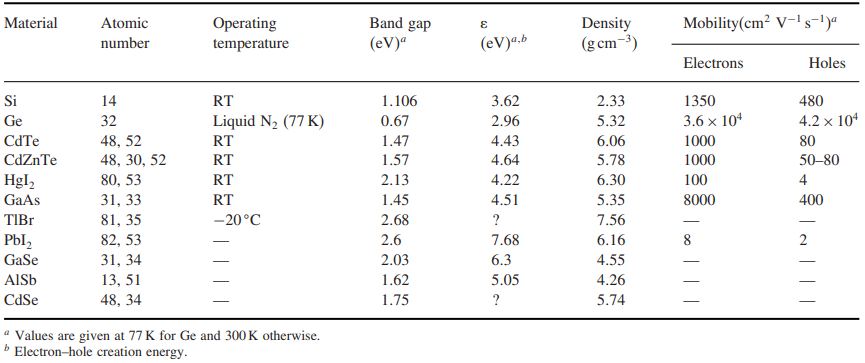
\includegraphics[width=\textwidth]{plots/candidates.png}
    \end{column}
    \begin{column}[c]{0.48\textwidth}
      \begin{itemize}
        \item Silicon: highly pure, low-priced, low atomic number (low energy photons)
        \item Germanium: higher Z -> good for higher energy gamma radiation
        \item low temperature -> reduce leakage current
        \item improvements reduced resolution to $\approx$ 1.8 keV
      \end{itemize}
    \end{column}
  \end{columns}
\end{frame}

\begin{frame}\frametitle{Semiconductor detector (Germanium)}
  \begin{columns}
    \begin{column}[c]{0.48\textwidth}
      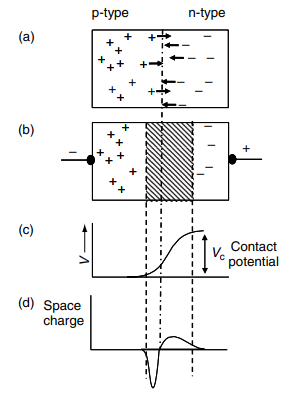
\includegraphics[width=\textwidth]{plots/junction.png}
    \end{column}
    \begin{column}[c]{0.48\textwidth}
      \begin{itemize}
        \item p-type, n-type germanium (3 and 5 valent impurities)
        \item electrons and holes recombine by diffusion -> depletion zone
        \item -> only local donator and acceptor hulls remain
        \item goal: seperation via external field inside depletion zone
        \item maximising the depletion zone -> hinder recombination -> reconstruct energy of the event
        \item probability of thermal excitation: $p(T) = T^{3/2} exp(-E_g / 2 k_b T)$ (background)
        \item p-n or M-S junctions possible
      \end{itemize}
    \end{column}
  \end{columns}
\end{frame}

\begin{frame}\frametitle{The Ge-detector}
  \begin{columns}
    \begin{column}[c]{0.48\textwidth}
      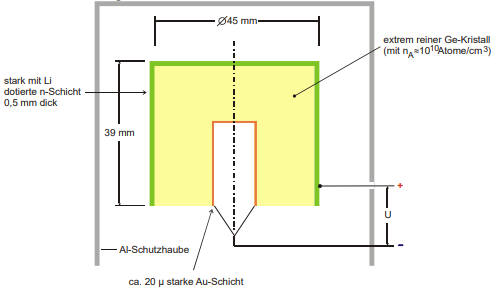
\includegraphics[width=\textwidth]{plots/ge.png}
    \end{column}
    \begin{column}[c]{0.48\textwidth}
      \begin{itemize}
        \item Aluminium casing as VETO region (40 - 50 keV)
        \item Lithium doped outside: connecting rreverse voltage
        \item inside steamed with gold (M-S junction)
        \item electronic signal: spectrum-histogram from Multichannel analyzer (MCA)
      \end{itemize}
    \end{column}
  \end{columns}
\end{frame}

\begin{frame}\frametitle{Metal-Semiconductor junction (n-Si)}
  \begin{columns}
    \begin{column}[c]{0.48\textwidth}
      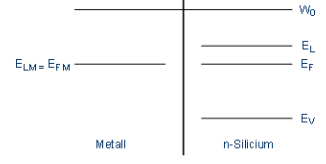
\includegraphics[width=0.7\textwidth]{plots/pre_m_s.png}
    \end{column}
    \begin{column}[c]{0.48\textwidth}
      \begin{itemize}
        \item $W_0$: vacuum level, $E_L$: conduction band, $E_F$: fermi energy
        \item $E_V$: valence band, $E_{LM}$: energy level in metal, $E_{FM}$: fermi energy in metal
        \item electrons can migrate from Semiconductor to metal since E-level is lower
        \item probability of finding electrons in conduction band gets lower
      \end{itemize}
    \end{column}
  \end{columns}
\end{frame}

\begin{frame}\frametitle{Metal-Semiconductor junction (n-Si)}
  \begin{columns}
    \begin{column}[c]{0.48\textwidth}
      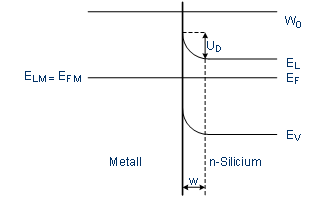
\includegraphics[width=0.7\textwidth]{plots/post_m_s.png}
    \end{column}
    \begin{column}[c]{0.48\textwidth}
      \begin{itemize}
        \item migrated charge carriers form depletion zone and lower fermi level
        \item additional $e^{-}$ must overcome the Schottky-barrier to flow into Metal
        \item fermi levels in metal and semiconductor equalize via diffusion process
      \end{itemize}
    \end{column}
  \end{columns}
\end{frame}

\begin{frame}\frametitle{Why is this junction used over p-n?}
  \begin{itemize}
    \item Si-Schottky diodes are substantially faster changing from forward bias to reverse bias
    \item -> switching action: 10 - 100 GHz possible because no moving "holes" in metal
    \item low forward voltage drop (0.15 - 0.45V) p-n: 0.6 - 0.75 V
    \item But: higher reverse leakage current
  \end{itemize}
\end{frame}

\begin{frame}\frametitle{Separation efficiency}
  \begin{itemize}
    \item minimal distance of 2 signals to register both
    \item Full Width at Half Maximum $\Delta E_{1/2} \approx 2.35 \sqrt{F E_\gamma \epsilon}$
    \item Fano factor of germanium $F = 0.1$
  \end{itemize}
\end{frame}

\begin{frame}\frametitle{Energy spectra}
  \begin{figure}
    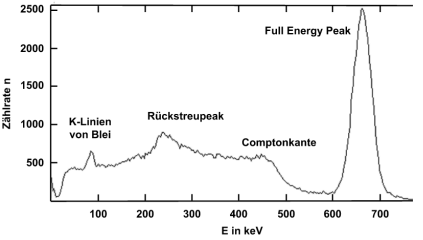
\includegraphics[width=0.8\textwidth]{plots/full_spec.png}
    \caption{Full spectrum of Cs-137 source}
  \end{figure}
\end{frame}

\begin{frame}\frametitle{Evaluation of gamma spectroscopy}
  \begin{columns}
    \begin{column}[c]{0.48\textwidth}
      PRO:
      \begin{itemize}
        \item quite cheap in material costs
        \item relatively fast result evaluation
        \item multinuclide analysis (distinct lines visible for all nuclides)
        \item non-destructive for emitter (radiation hardness of detector given)
        \item remote measurement
      \end{itemize}
    \end{column}
    \begin{column}[c]{0.48\textwidth}
      CONTRA:
      \begin{itemize}
        \item often less sensitive
        \item require large sample masses (if not gamma rays from space)
      \end{itemize}
    \end{column}
  \end{columns}
\end{frame}

\begin{frame}\frametitle{Applications}
  \begin{itemize}
    \item medical application: positron emission tomography (PET) [tumor therapy]
    \item -> positron-emitting pharmaceutical injection near tumor -> imaging through 511 keV lines
    \item security scans for explosives
    \item monitoring nuclear waste
  \end{itemize}
\end{frame}

\begin{frame}
  \begin{itemize}
    \item \textbf{Thank you for listening!}
    \item Questions?
    \item Comments?
  \end{itemize}
\end{frame}

\begin{frame}\frametitle{Quellen}
\url{https://onlinelibrary.wiley.com/doi/book/10.1002/9780470861981} \\
\url{V18_Anleitung.pdf} \\
\url{https://www.nrc.gov/docs/ML1122/ML11229A699.pdf} \\
\url{https://www.electrical4u.com/schottky-diode/} \\
\end{frame}

\begin{frame}\frametitle{Backup}
  \begin{columns}
    \begin{column}[c]{0.45\textwidth}
      \begin{itemize}
        \item Attenuation egde for caesium iodine (CsI)
        \item 2 K-lines and 2 L-lines
      \end{itemize}
    \end{column}
  \begin{column}[c]{0.45\textwidth}
    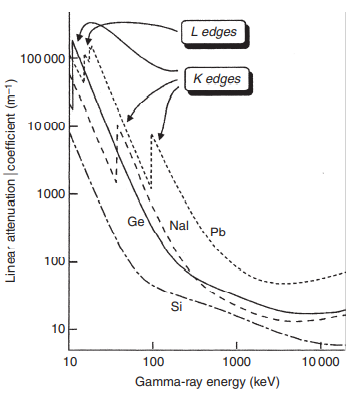
\includegraphics[width=0.8\textwidth]{plots/attenuation_edges.png}
  \end{column}
  \end{columns}
\end{frame}

\end{document}
